% @Author: Taha Bouhsine


%%%%%%%%%%%%%%%%%%%%%%%%%%%%
% CHAPTER                  %
%%%%%%%%%%%%%%%%%%%%%%%%%%%%
\setcounter{mtc}{9}
\chapter{Analysis And Design}%
\label{chap:chapter_two}
\minitoc
%%%%%%%%%%%%%%%%%%%%%%%%%%%%
% SECTION                  %
%%%%%%%%%%%%%%%%%%%%%%%%%%%%
Among all the stages of the product's life cycle, the design stage contributes significantly to the improvement of competitiveness, because it permits reduction of costs and often, shortening of the time necessary to get the solutions to the production stage.

\section{General description of the platform}
Sahem is a unique crowdfunding app built primarily in MEAN Stack technologies. It has one type of user that can be two types at the same time: can be either a creator or a funder. A funder donates while a creator acquires the fund. This app has a trust-building mechanism called corroboration where funders can certify creators and allow creators to certify their claims through uploading documentary proofs in an image format. The final mode of crowdfunding takes place through the exchange of transactional information where Funders can pay and amount of monetary by a bank transfer or by card.
We took the chance in providing easy accessibility to the main functionalities of the platform, as we tried to ask what is the most thing that a user wants to do, and we tried to optimize the number of clicks that a user would have to make in order to do the actions he wants, so we sought to make both of the creation of a fundraiser, and funding a project accessible by a maximum of 3 clicks and after the creator starts a fundraiser he can directly share a link that can lead to the funding page, bypassing the project description and content, to help in making the funders fund in a very short time, instead of filling unnecessary forms and passing by multiple pages.

\section{Specification of requirements}
We will proceed according to the UML method which consists of identifying and modeling the various business processes in order to easily migrate to an object architecture from a static and dynamic point of view. This analysis presents a total abstraction being independent of any technology or implementation.

The specification of the needs will allow us to have a better approach of the users, the functionalities, and the relationship between the two. It will be in the form of a use case. For this we will proceed as follows:

\begin{itemize}\addtolength{\itemsep}{-0.35\baselineskip}   
      \item 
      Identification of requirements.
      \item 
      Identification of the actors of the system.
      \item 
      Identification of use cases.
      \item 
      Description of use cases.
      \item 
      Grouping of use cases into packages.
\end{itemize}


\subsection{Requirements}
The requirements that we have put on the end-product were divided into basic functionalities and optional functionalities.
The User’s basic functionalities are:
\begin{enumerate}
    \item
          Account management: Create an account, login, profile, settings, personal info,
          personal dashboard.
    \item
          Start a campaign: send in a proposal for a Fundraiser (webform).
    \item
          Share function: functionality so that a campaign can be shared within social networks, such as Facebook, Instagram, LinkedIn, Twitter, and potentially Pinterest and Google.
    
    \item
          Payment function: Funders should be able to pay their ticket through Credit Card.
    \item
          Review function: Funders should have the opportunity to give reviews about and react to events
          that have taken place.
    \item
          Countdown timer: a timer that shows how much time a campaign has left until it closes.
    \item
          Current overview: each campaign should show for example the number of tickets sold/amount of investors, the amount of money raised so far and the goal amount to be raised.
\end{enumerate}


The User’s optional functionalities are:

\begin{enumerate}
      \item
          Contribution invitation: functionality to send out concrete requests to contribute a certain amount
          within the personal social network.
    \item
          Personalized recommendations (recommender system): the system will advise, suggest, or give concrete offers. Logged-in visitors see a personalized recommendation based on social profiles and the
          platform’s web page content and actions.
    \item
          Share option via Whatsapp
    \item
          Online helpdesk: chat possibility with a helpdesk worker.
    \item
          Communication tools: communication possibilities with other members and/or the organization of an
          event via chat.
    \item
          Connection with social media: e.g. Facebook application for special opportunities and/or campaigns
          that enabled even more interaction with the target group.
    \item
          Social login: login with a social account.
    \item
          Wallet: deposit money in your wallet, which enables you to make several contributions by
          paying with the money in your wallet.
    \item
          Recruit function: a tool to gather more contributors. A contributor can share a campaign within their
          own social networks.
    \item
          Notifications: reminders and/or messages related to upcoming events and updates of events.
    \item
          Mobile App: extra functionalities through the use of a camera and GPS on the actual event: e.g. picture/video upload to the website or live visitor numbers.

    \item
          Agenda/calender: an overview that shows which events will take place on which dates (including events
          that have already taken place).
    \item
          Newsletter: send an overview of the events to members of the platform community or a certain
          selection.
    \item
          Promotion function: functionality to share and promote events on different levels: community (everyone), events (only participants of a specific event), social media (within social networks).
    \item
          Campaign management: management tools for the event organization.
    \item
          Reports/statistics: data analyses, tools for advanced analysis of the web page visits.
\end{enumerate}




\subsection{Identification of actors}
In UML we don't use the term users but actors. A player in a system is an entity external to this system that interacts (data entry, reception of information, etc.) with it. The actors make it possible to define the interface that the system will offer to its environment. And also the actor groups together several users who have the same role. And to define actores it will be necessary to identify their roles.
To facilitate identification, we can imagine this: everything that is outside and interacts with the system is an actor, everything that is inside is a functionality to be realized.
The different actors of the studied system are as Figure \ref{fig:sahemactors} shows:

\begin{enumerate}
    \item  Creator.
    \item  Funder will be merged with Creator.
    \item  Administrator.
    \item  Visitor.
\end{enumerate}

\begin{figure}[!ht]
      \centering
      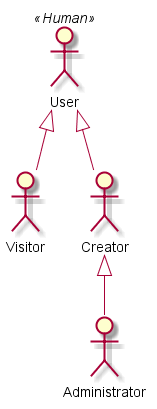
\includegraphics[scale=0.6]{assets/Actors.png}
      \caption{Sahem Platform's Actors}
      \label{fig:sahemactors}
\end{figure}
\subsection{Identification of objectives and use cases}
A use case described in the form of actions and reactions, the behavior of a system from a user point of view. It must add value to the actor concerned. Each use case contains a list of functionalities that will be detailed in the following section.

We will first determine the objectives that will allow us to deduce the use cases and all this in Table \ref{tab:id_objec_uc}:
\begin{longtable}{|m{10em}|m{10em}|m{10em}|}\hline
Management & Functionalities        &   Sub-functionalities                        \\\hline
    \multirow{4}{*}{Administration} & \multirow{2}{*}{Authentication}       & Authentication                          \\\cline{3-3}
                                               &                                       & Registration                            \\\cline{2-3}
                                               & \multirow{5}{*}{User Maintainance}    & Add User                                \\\cline{3-3}
                                               &                                       & Modify User                             \\\cline{3-3}
                                               &                                       & Delete User                             \\\cline{3-3}
                                               &                                       & Consult the information of a user       \\\cline{3-3}
                                               &                                       & Show the list of users                  \\\cline{2-3}
                                               & \multirow{2}{*}{Roles}                & Show users by roles                     \\\cline{3-3}
                                               &                                       & Modify a user's role                    \\\cline{2-3}
                                               & \multirow{1}{*}{Statistics}           & Access the statistics of the plateforme \\\hline
    \multirow{4}{*}{Fundraiser}    & \multirow{3}{*}{Creator's Monitoring} & Personal information modification       \\\cline{3-3}
                                               &                                       & Access a creator profile                \\\cline{3-3}
                                               &                                       & Desactivate an Account                  \\\cline{2-3}
                                               & \multirow{2}{*}{Funds Monitoring}     & Fund a project                          \\\cline{3-3}
                                               &                                       & Confirm funding a project               \\\cline{3-3}
                                               &                                       & List of previous funds                  \\\cline{2-3}
                                               & \multirow{6}{*}{Projects Monitoring}  & Create a project                        \\\cline{3-3}
                                               &                                       & Edit a project                          \\\cline{3-3}
                                               &                                       & Delete a project                        \\\cline{3-3}
                                               &                                       & Like a project                          \\\cline{3-3}
                                               &                                       & Share a project                         \\\cline{3-3}
                                               &                                       & Comment on a project                    \\\cline{2-3}
                                               & \multirow{2}{*}{Search}               & Search a project by name                \\\cline{3-3}
                                               &                                       & Show Fundraisers by category            \\\hline
    \multirow{2}{*}{Payment}        & \multirow{1}{*}{Billing}              & Show the bill                           \\\cline{2-3}
                                               & \multirow{1}{*}{Online Payment}       & Choose payment method                   \\\hline

    \caption{Identification of objectives and use cases}
    \label{tab:id_objec_uc}
\end{longtable}

%%%%%%%%%%%%%%%%%%%%%%%%%%%%
% SECTION                  %
%%%%%%%%%%%%%%%%%%%%%%%%%%%%
\section{Functional Analysis}
Functional analysis is a methodology for analyzing the mission and performance requirements of a system, and translating them into discrete activities or tasks which must be performed by the system. Determination of the system's functionality is the first step in obtaining a conceptual view of a system that is to be designed.

Figure \ref{fig:globaluc} showcase the general use case of a user in Sahem System. And is more detailed in Figure \ref{fig:fund project ucs}, Figure \ref{fig:user with projects ucs}, and Figure \ref{fig:user authentication and account management ucs}. 
\begin{figure}[!ht]
      \center
      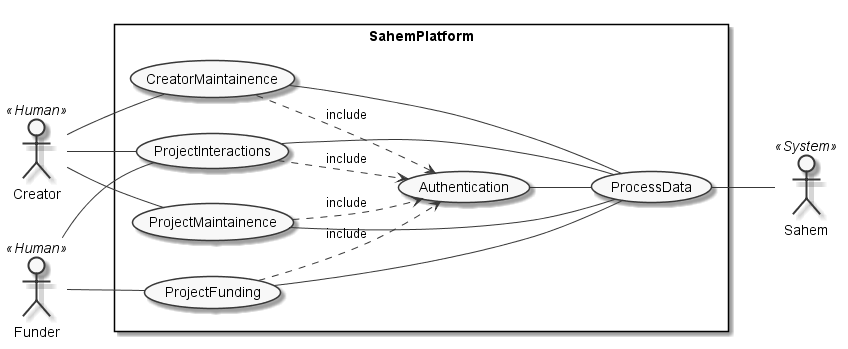
\includegraphics[scale=0.5]{assets/global.png}
      \caption{Sahem System Global Use Case}
      \label{fig:globaluc}
\end{figure}


% 

\begin{figure}
      \centering
      \begin{subfigure}[b]{0.45\textwidth}
          \centering
          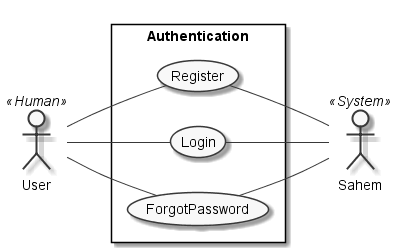
\includegraphics[width=\textwidth]{assets/user_maintainence.png}
          \caption{Authentication Use Case}
          \label{fig: authentication uc}
      \end{subfigure}
      \hfill
      \begin{subfigure}[b]{0.45\textwidth}
          \centering
          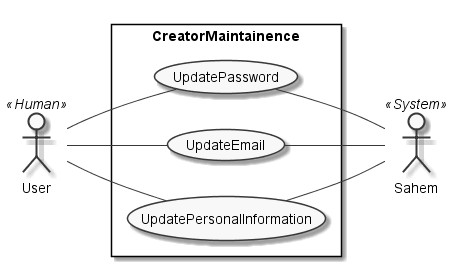
\includegraphics[width=\textwidth]{assets/CreatorMaintainence.png}
          \caption{Account Maintainance Use Case}
          \label{fig:account maintainence uc}
      \end{subfigure}
         \caption{User’s Authentication and Account Management}
         \label{fig:user authentication and account management ucs}
 \end{figure}



\begin{figure}
      \centering
      \begin{subfigure}[b]{0.45\textwidth}
          \centering
          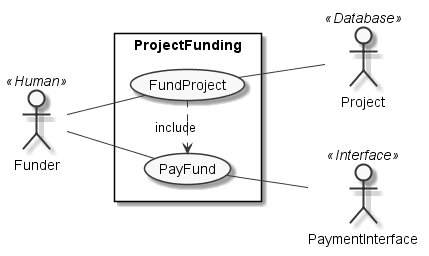
\includegraphics[width=\textwidth]{assets/FundingProject.png}
          \caption{Fund Project Use Case}
          \label{fig:funding project uc}
      \end{subfigure}
      \hfill
      \begin{subfigure}[b]{0.45\textwidth}
          \centering
          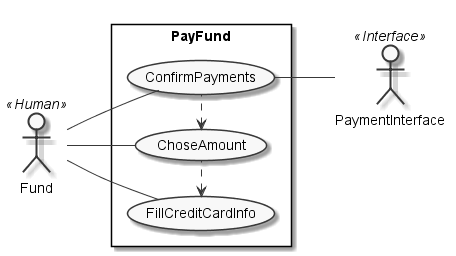
\includegraphics[width=\textwidth]{assets/UC31-PayFund.png}
          \caption{Paying Use Case}
          \label{fig:paying funds uc}
      \end{subfigure}
         \caption{Funding Projects Use Cases}
         \label{fig:fund project ucs}
 \end{figure}

 \begin{figure}
      \centering
      \begin{subfigure}[b]{0.45\textwidth}
          \centering
          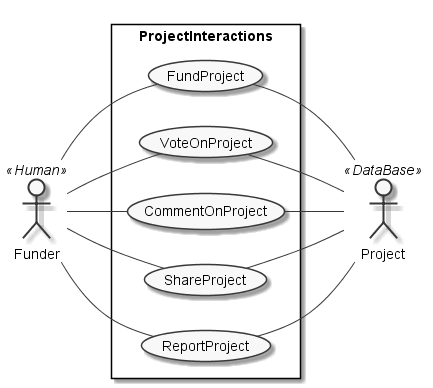
\includegraphics[width=\textwidth]{assets/ProjectInteractions.png}
          \caption{Project interactions Use Case}
          \label{fig:project interactions uc}
      \end{subfigure}
      \hfill
      \begin{subfigure}[b]{0.45\textwidth}
          \centering
          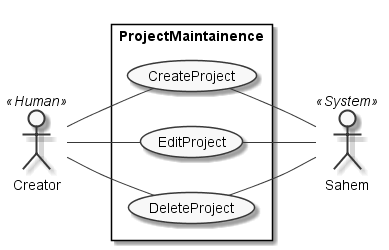
\includegraphics[width=\textwidth]{assets/ProjectMaintainence.png}
          \caption{Project Maintainance Use Case}
          \label{fig:project maintainence uc}
      \end{subfigure}
         \caption{User’s interactions with projects Use Cases}
         \label{fig:user with projects ucs}
 \end{figure}

% \begin{figure}[!ht]
%       \center
%       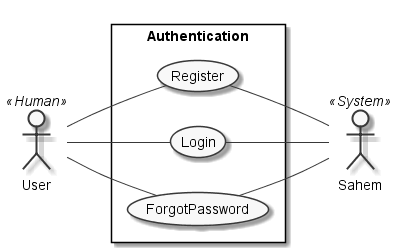
\includegraphics[scale=0.40]{assets/user_maintainence.png}
%       \label{fig:qweq}
%       \caption{Authentication Use Case}
% \end{figure}

% \begin{figure}[!ht]
%       \center
%       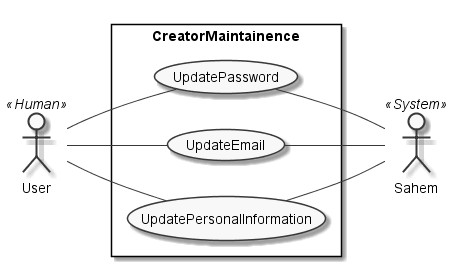
\includegraphics[scale=0.40]{assets/CreatorMaintainence.png}
%       \label{fig:qweq}
%       \caption{Account Maintainance Use Case}
% \end{figure}

% \begin{figure}[!ht]
%       \center
%       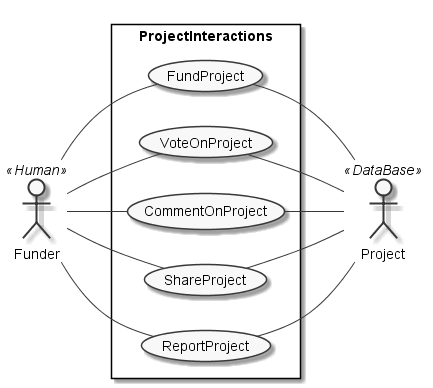
\includegraphics[scale=0.40]{assets/ProjectInteractions.png}
%       \label{fig:qweq}
%       \caption{Project interactions Use Case}
% \end{figure}

% \begin{figure}[!ht]
%       \center
%       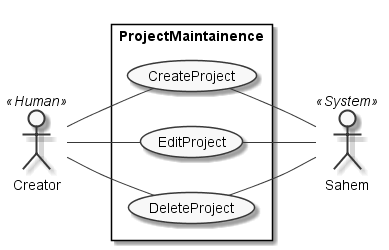
\includegraphics[scale=0.40]{assets/ProjectMaintainence.png}
%       \label{fig:qweq}
%       \caption{Project Maintainance Use Case}
% \end{figure}

% \begin{figure}[!ht]
%       \center
%       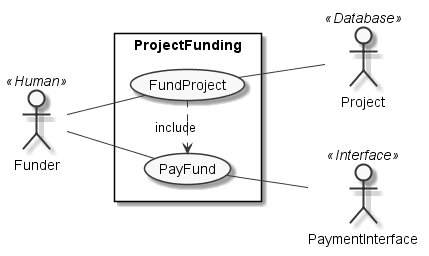
\includegraphics[scale=0.40]{assets/FundingProject.png}
%       \label{fig:qweq}
%       \caption{Fund Project Use Case}
% \end{figure}

% \begin{figure}[!ht]
%       \center
%       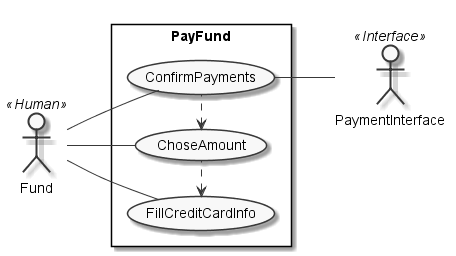
\includegraphics[scale=0.40]{assets/UC31-PayFund.png}
%       \label{fig:qweq}
%       \caption{Paying Use Case}
% \end{figure}

\clearpage
%%%%%%%%%%%%%%%%%%%%%%%%%%%%
% SECTION                  %
%%%%%%%%%%%%%%%%%%%%%%%%%%%%
\section{Dynamic Analysis}
Dynamic analysis is the testing and evaluation of a program by executing data in real-time. The objective is to find errors in a program while it is running, rather than by repeatedly examining the code offline.
By debugging a program in all the scenarios for which it is designed, dynamic analysis eliminates the need to artificially create situations likely to produce errors. Other advantages include reducing the cost of testing and maintenance, identifying and eliminating unnecessary program components.

First of all, we start by creating an activity diagram, that summarizes the life cycle of all the user's interactions with the Sahem system (Figure \ref{fig:activity diagram}), then we created different Sequence diagrams modeling the different functionalities of Sahem system and the interactions between its components (Figures \ref{fig:authentication seq}, \ref{fig:PostProject seq}, \ref{fig:project seq}, and \ref{fig:projects seq}).

\begin{figure}[!ht]
      \center
      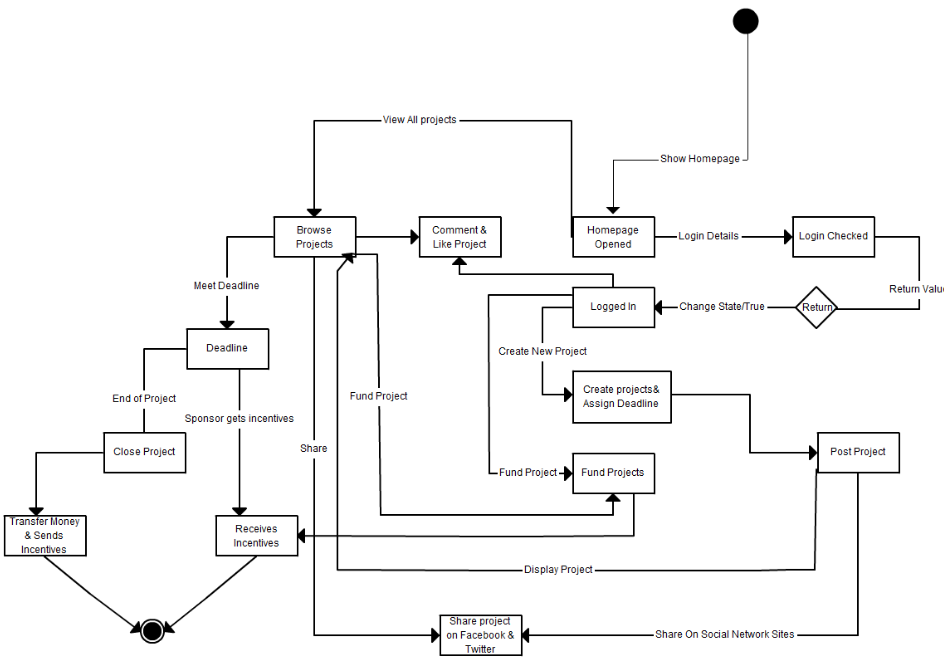
\includegraphics[scale=0.51]{assets/activity.png}
      \caption{Sahem Activity Diagram}
      \label{fig:activity diagrma}
\end{figure}

\begin{figure}[!ht]
      \center
      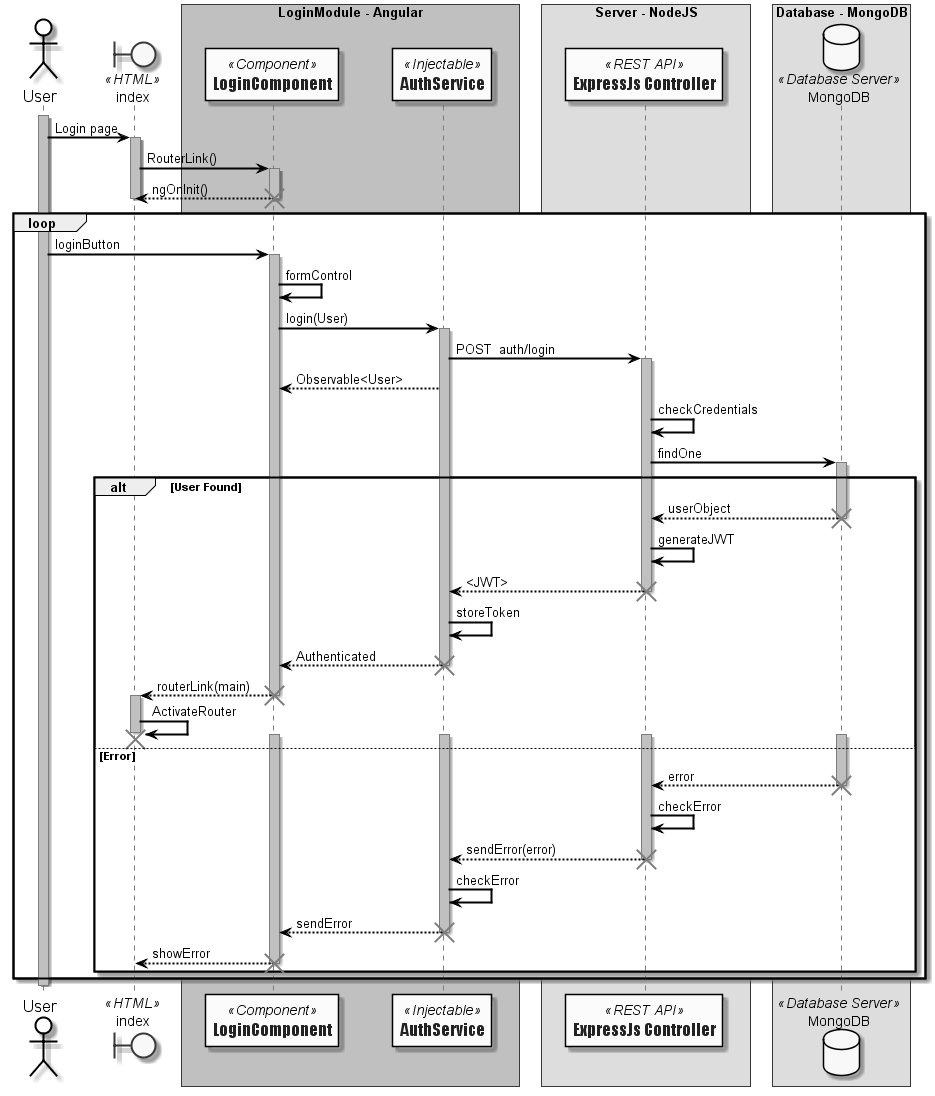
\includegraphics[scale=0.45]{assets/authentication.png}
      \caption{User Authenticating Sequence Diagram}
      \label{fig:authentication seq}

\end{figure}

\begin{figure}[!ht]
      \center
      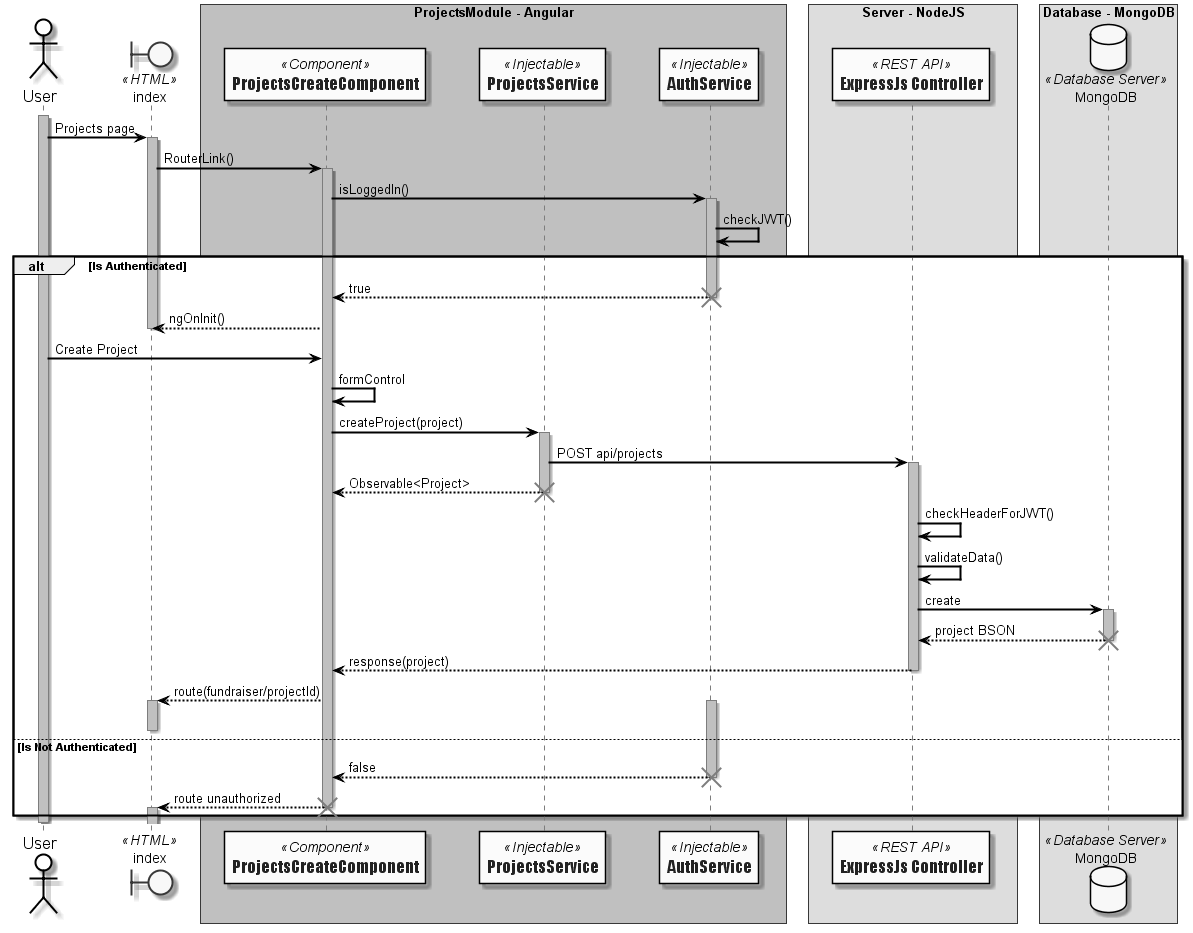
\includegraphics[scale=0.35]{assets/PostProject.png}
      \caption{Create a Project Sequence Diagram}
      \label{fig:PostProject seq}

\end{figure}

\begin{figure}[!ht]
      \center
      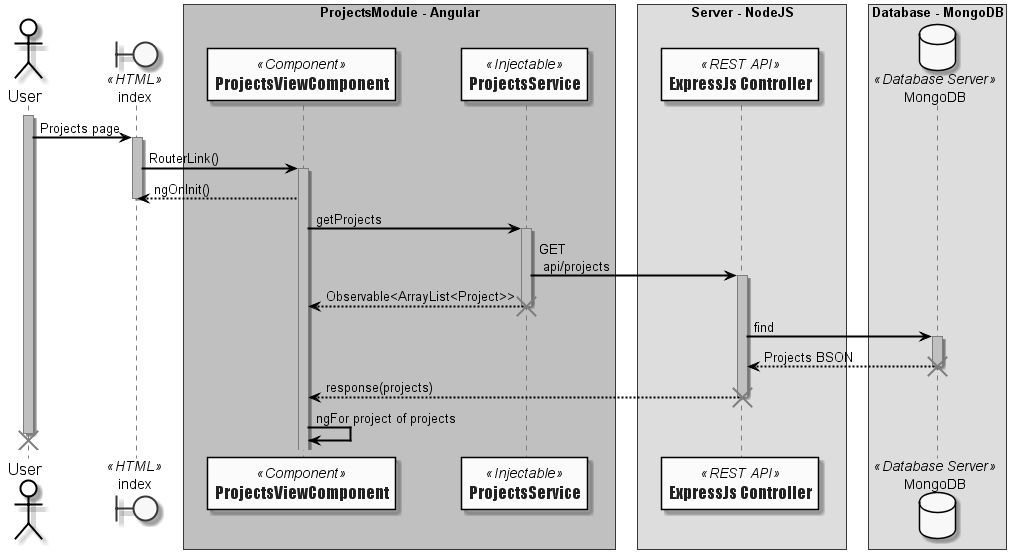
\includegraphics[scale=0.40]{assets/projects.png}
      \caption{Get Projects Sequence Diagram}
      \label{fig:projects seq}

\end{figure}

\begin{figure}[!ht]
      \center
      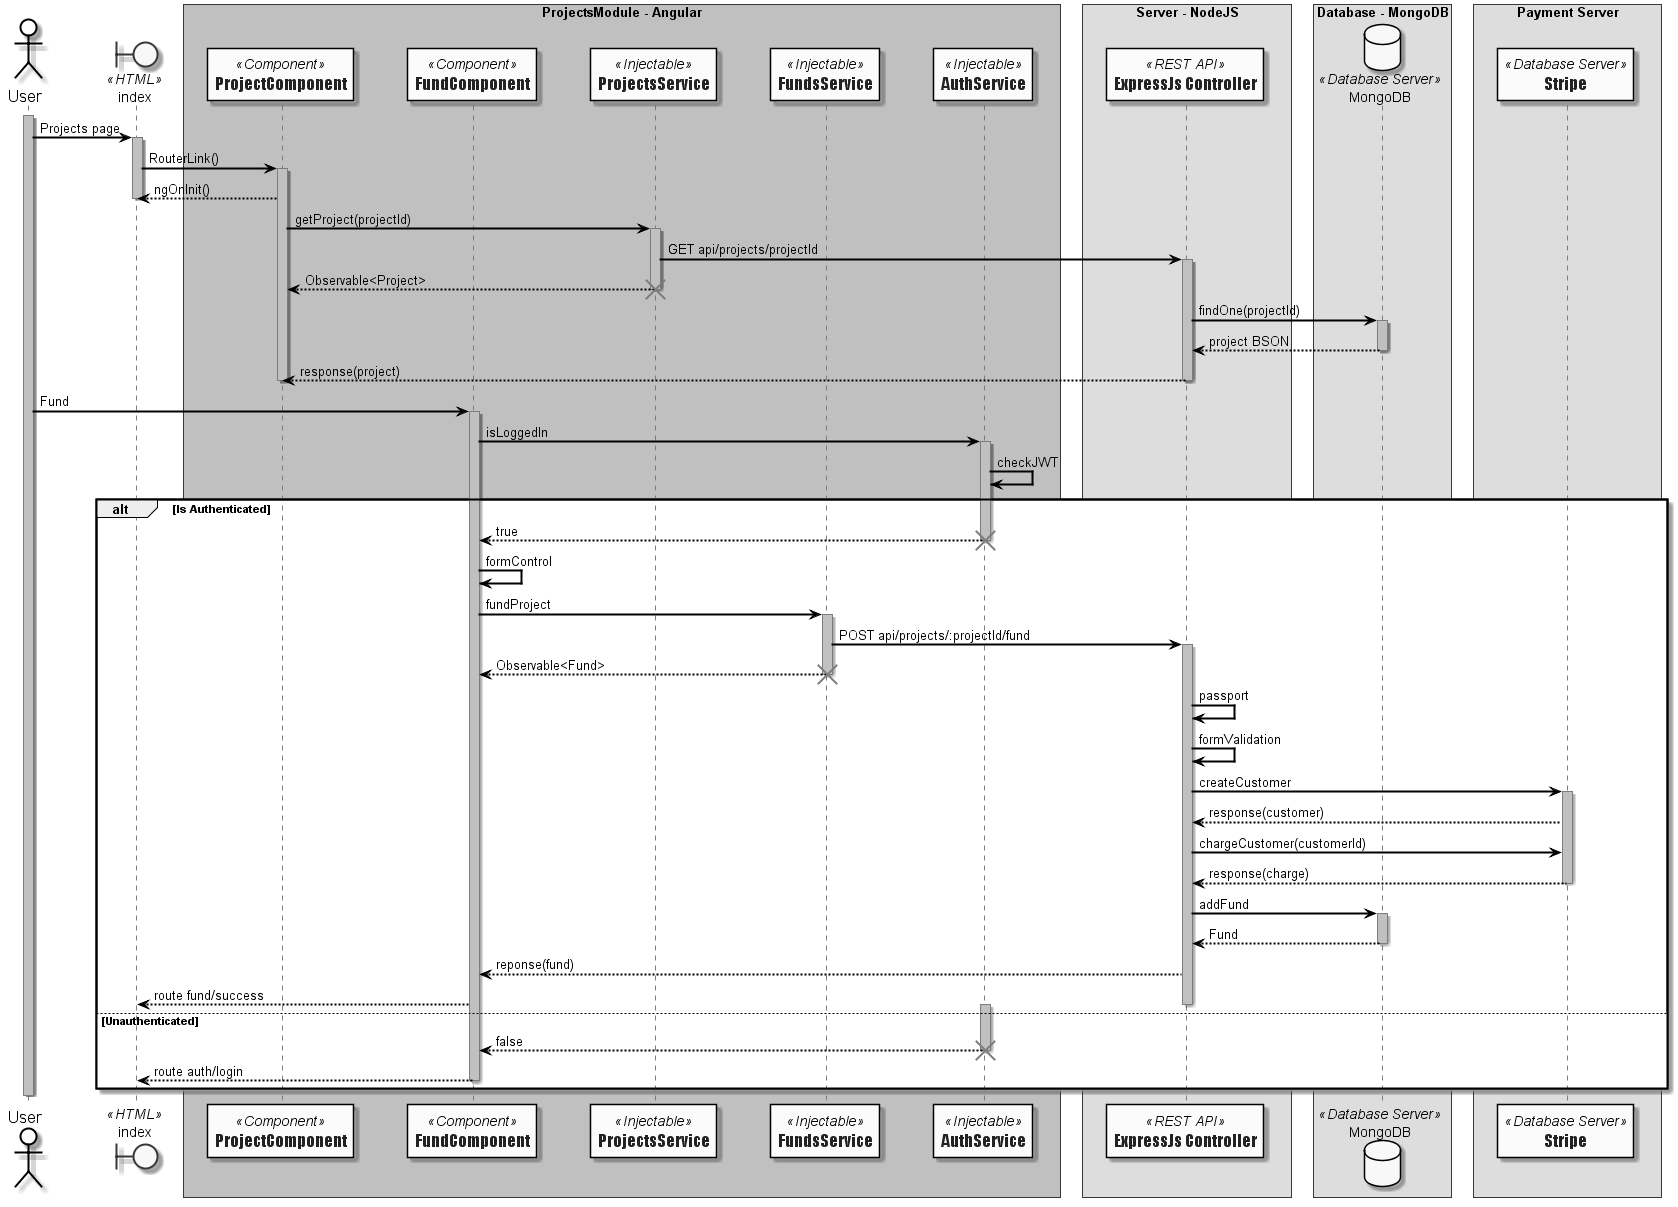
\includegraphics[scale=0.37,angle=90]{assets/project.png}
      \caption{Get And Fund Project Sequence Diagram}
      \label{fig:project seq}

\end{figure}
%%%%%%%%%%%%%%%%%%%%%%%%%%%%
% SECTION                  %
%%%%%%%%%%%%%%%%%%%%%%%%%%%%
\clearpage
\section{Structured Analysis}
Structured Analysis is a development method that allows the analyst to understand the system and its activities logically.

It is a systematic approach, which uses graphical tools that analyze and refine the objectives of an existing system and develop a new system specification that can be easily understandable by the user.


\begin{figure}[!ht]
      \center
      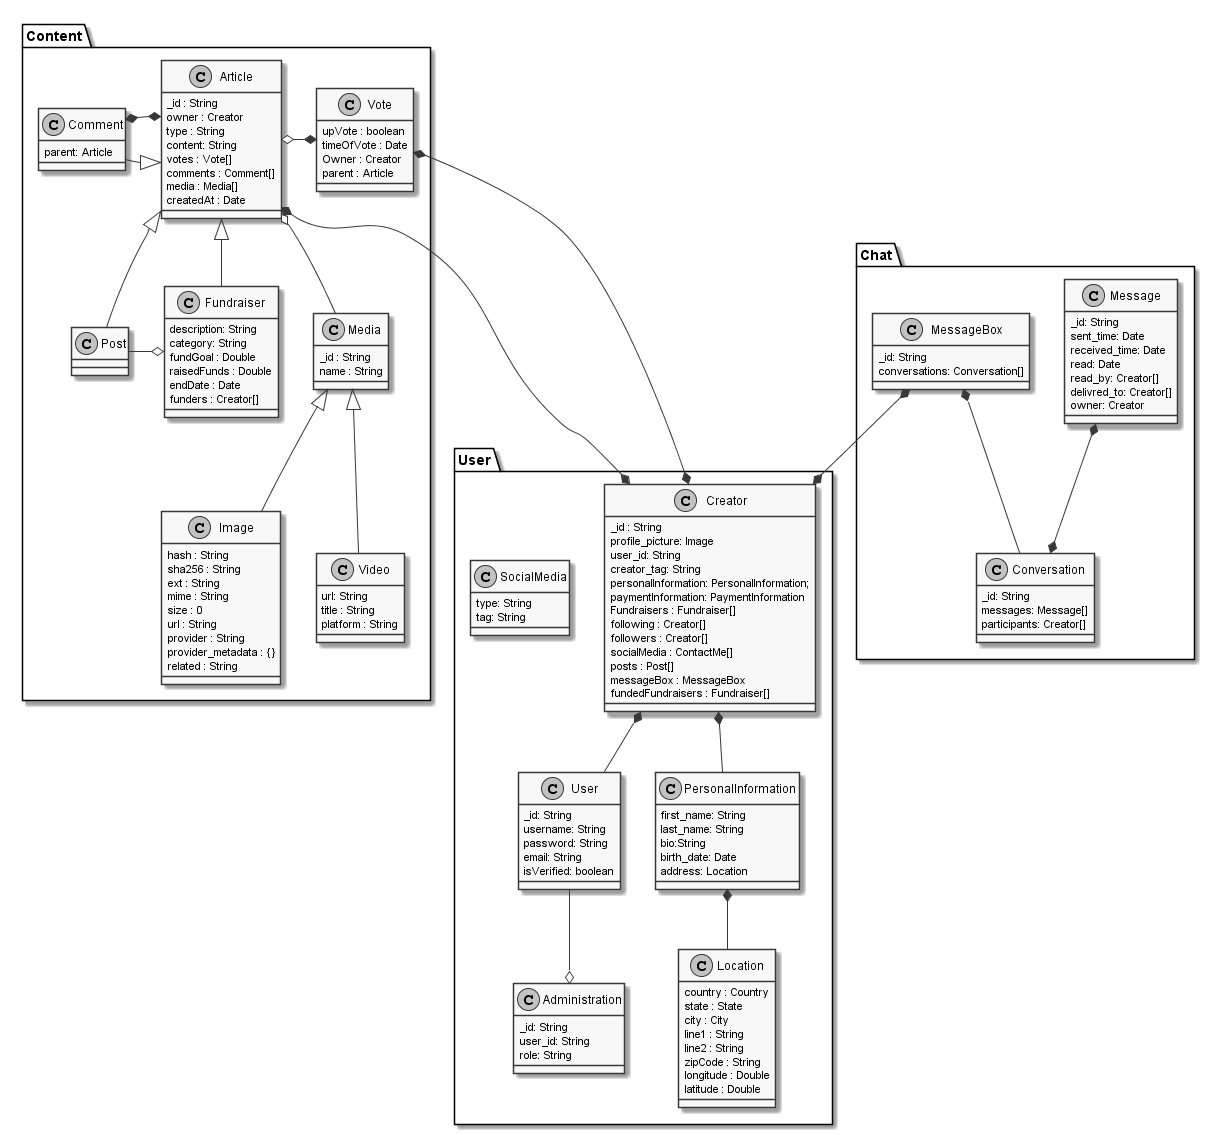
\includegraphics[scale=0.40,angle=90]{assets/User.png}
      \label{fig:qweq}
      \caption{Sahem Class Diagram}
\end{figure}


